\chapter[Structured Visual Model Learning]{Structured Dictionary Learning and Feature Encoding}
\label{ch_groupsparse}

\begin{singlespace*}
\begin{abstract}
 \scriptsize{\textbf{Chapter abstract:} Sparse, redundant representations offer a powerful emerging model for signals and images \citep{Mairal2008,Yang2009}. This model approximates a data vector as a linear combination of a subset of basis elements from a learnt over-complete basis set. The combination is a sparse selection of basis elements. Sparsity is induced by adding a regularization constraint to the coefficients in the loss function. The degree of sparsity is typically determined empirically. A $\ell_{0}$ or $\ell_{1}$-norm is used to regularize the coefficients. This effective approach however considers each basis element individually. It does not utilize prior information of structure within the basis set and disregards possible groups of basis elements. In this chapter, sparse coding is augmented with structure learnt from co-clustering in terms of groups of semantically related basis elements. In the first part, a structured multiple manifold dictionary is learnt using co-clustered sub-spaces with Structured Sparse Principal Component Analysis (SSPCA) \citep{Jenatton2009}. It builds upon Sparse-PCA \citep{Zou2004} where the sparse selection of sub-spaces to represent a feature vector is independent of semantic significance of the selected sub-spaces. The second part deals with learning structured feature encoding. Typically, the Lasso which uses $\ell_{1}$-norm regularization is used for sparse selection of dictionary elements. To incorporate a prior structure, the group Lasso which uses $\ell_{2,1}$ mixed norm regularization \citep{zibulevsky2010} is used for sparse selection of groups of semantically related dictionary elements. Both structured sparse visual models are shown to improve performance over their corresponding regular sparse visual models.
 }
\end{abstract}
\end{singlespace*}

\section[Introduction]{Introduction}
\label{ch_groupsparse_sec_introduction}

In this chapter, semantically relevant structure that was estimated in previous chapters is incorporated in learning a visual model. The method selected for this is sparse coding. Sparsity inducing algorithms for learning a visual model have enjoyed much success in recent years \citep{Yang2009}. They have the ability of simultaneous feature selection and model learning. One explanation for their notable performance is their ability to deal with intra-category appearance variation. Consider typical training feature data. It contains more elements than is required to represent any instance of any visual category. For example, the estimated intrinsic dimensionality of $128$-dimensional feature vectors is in the neighbourhood of $14$, based on the empirical results in \cref{ch_dictionary_subsec_intrinsicdimensionality}. The methods discussed in previous chapters first compute a single subset of all the sub-spaces. All the elements of this subset are subsequently used to represent every feature descriptor. However, a visual category consists of distinct parts, and each part spans a different subset of the basis set. A single subset can not satisfactorily accommodate the variation in appearance found in a visual category. In other words, regardless of the efficacy of the sub-space embedding technique, a single sub-manifold is inappropriate for all feature descriptors. A conceptual illustration of this is shown in \cref{fig:objectpartsubspace}. Different parts of the visual object `car' are embedded in different sub-manifolds due to their distinct local patch structure. A single sub-manifold can not account for all `car' parts. Sparsity inducing methods on the other hand, do not select a subset of basis elements a priori. A feature descriptor is assigned its own subset of basis elements. Although the cardinality of the subset in both, sparse coding and previously discussed methods may be the same, it is the ability for individual subset selection that makes sparse coding better suited to model intra-category 
appearance variation.

\begin{figure}
 \centering
 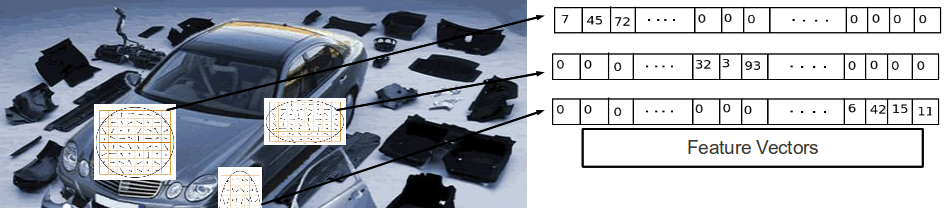
\includegraphics[width=\textwidth]{./GroupSparse/figures/subspace.png}
 \caption[Conceptual illustration of relation between object part and descriptor sub-space]{Conceptual illustration of relation between object part and descriptor sub-space. Different parts of a `car' due to the local image structure are embedded in different sub-manifolds in feature space. A single sub-manifold can not satisfactorily model all three `car' parts.}
 \label{fig:objectpartsubspace}
\end{figure}

Stated formally, the aim of sparse coding is to find a set of basis vectors $\{ \mathbf{d}_{1}, \ldots, \mathbf{d}_{r} \}$ such that an input image $\mathbf{Z} \in \mathds{R}^{p \times n}$ can be represented as a linear combination of these basis vectors $\mathbf{Z} = \sum_{i=1}^{r} \alpha_{i} \mathbf{d}_{i}$. While techniques such as PCA learn a complete set of basis vectors efficiently, the aim is to learn an over-complete set of basis vectors to represent input images. The elements of an over-complete basis are better able to capture structures and patterns inherent in the input data. However, with an over-complete basis, the coefficients $\alpha_{i}$ are no longer uniquely determined by the input vector $\mathbf{Z}$. Therefore, in sparse coding, the additional criterion of sparsity is utilized to resolve the degeneracy introduced by over-completeness. In the experiments in previous chapters, a `universal' dictionary had been learnt from a corpus of all visual categories in a dataset\footnote{This choice of dictionary is in contrast to learning a `category specific' dictionary}. A universal dictionary is an over-complete dictionary, as it contains elements from multiple visual categories. 

The data matrix $\mathbf{Z} \in \mathds{R}^{p \times n}$ is factorized to dictionary matrix $\mathbf{D} \in \mathds{R}^{p \times r}$, and coefficient matrix $\mathbf{A} \in \mathds{R}^{p \times n}$, with a sparse regularization constraint $\Omega$ on the columns of the coefficient matrix. Sparse coding methods solve the following regularized problem

\begin{equation} \label{eq:losssparsecoding}
 \min_{\alpha} \frac{1}{n} \sum_{i=1}^{n} L(\mathbf{z}_{i}, \mathbf{d} \alpha_{i}) + \lambda \Omega(\alpha)
\end{equation}

where $\lambda$ is a regularization parameter. The first term $\frac{1}{n} \sum_{i=1}^{n} L(\mathbf{z}_{i}, \mathbf{d} \alpha_{i})$ is called empirical risk or loss function. It is convex and continuously differentiable \citep{Jenatton2010}. Typical choices for $\Omega$ use the $\ell_{0}$-norm or $\ell_{1}$-norm. The regularized problem using the $\ell_{0}$-norm is

\begin{equation} \label{eq:l0normloss}
 \min_{\alpha} \frac{1}{n} \sum_{i=1}^{n} \parallel \mathbf{z}_{i} - \mathbf{D} \alpha_{i} \parallel^{2} + \lambda \parallel \alpha_{i} \parallel_{0}
\end{equation}

The use of $\ell_{0}$-norm forces selection of a subset of fixed cardinality. While this is conceptually appealing, efficient regularization methods that use $\ell_{0}$-norm are difficult to implement. The $\ell_{1}$-norm regularization on the other hand has become a popular tool. It profits from efficient algorithms \citep{Efron2004, Lee2007, Yuen2009} and a well developed theory for generalization properties and variable selection consistency \citep{Shen2013, Zhang2009}. The regularization problem using the $\ell_{1}$-norm is

\begin{equation} \label{eq:l1normloss}
 \min_{\alpha} \frac{1}{n} \sum_{i=1}^{n} \parallel \mathbf{z}_{i} - \mathbf{D} \alpha_{i} \parallel^{2} + \lambda \parallel \alpha_{i} \parallel_{1}
\end{equation}

Notwithstanding their notable performance, sparse coding methods have an issue. When regularizing by the $\ell_{1}$-norm, each variable is considered individually. The position of a variable in the input feature vector is disregarded. This means existing relationships and structures between the variables are ignored. However, using sparsity induction in learning a visual model could benefit from this type of prior knowledge. There are two reasons for including structural a priori information. One is improved predictive performance of the learnt model. The other is improved interpretability of the model. While the $\ell_{1}$-norm regularization succeeds in inducing sparsity, it does so without knowledge of the semantic relevance of the variables selected. Incorporating a priori structure can encourage the selection of variables with regard to their semantic relation to other variables.

For example, in the field of face recognition, robustness to occlusions can be increased by incorporating structure. The features are considered as sets of pixels that form small convex regions on the face images \citep{Jenatton2010}. A simple $\ell_{1}$-norm regularization can not encode this specific spatial locality constraint \citep{Jenatton2010}. Another example in the field of computer vision is object and scene recognition, where a goal is the computation of bounding boxes in images \citep{Harzallah2009}. They are detected by modelling the spatial arrangement of the pixels over the images. An unstructured sparsity-inducing regularization that disregards this spatial information is therefore not necessarily able to segment the image with bounding boxes as it may be modelling a mixture of object feature with background contextual features.

These examples motivate the need for sparsity-inducing regularization schemes, capable of encoding more sophisticated prior knowledge about the expected sparsity patterns. As mentioned above, the $\ell_{1}$-norm focuses only on cardinality and cannot easily specify information about the patterns of non-zero coefficients induced in the solution, since all non-zero patterns are theoretically possible. Group $\ell_{1}$-norms \citep{Yuan2006, Roth2008, Huang2009} consider a partition of all variables into a certain number of subsets and penalize the sum of the Euclidean norms of each one, leading to the selection of groups rather than individual variables. The consistency of group sparse method has been studied in \citep{Bach2008}.

Combining the ideas of sparse models and group structure from co-clustering, is work on structured sparsity induced matrix factorization \citep{Kim2012}. At its heart is a $\ell_{q,1}$-mixed norm where $q \in \{2, \ldots, \infty \}$, where typically $q = 2$ \citep{Liu2008a}. It achieves sparsity at the group level, where data elements within a group are treated equally using the $\ell_{2}$-norm, while sparsity is induced upon entire groups using the $\ell_{1}$-norm. The group Lasso \citep{Bach2008} is the $\ell_{2,1}$-norm regularization equivalent of Lasso \citep{Tibshirani1994} for $\ell_{1}$-norm regularization. During matrix factorization the matrices within each group are orthogonal.

In the previous chapter, co-clustering was utilized to estimate groups of sub-spaces and groups of dictionary elements. In this chapter, the estimated groups of sub-spaces are used in conjunction with structured sparse principal component analysis (SSPCA) to learn a group structured multiple-manifold dictionary, in \cref{ch_groupsparse_sec_manifold}. This dictionary is compared to a dictionary computed using regular sparse principal component analysis (SPCA). The empirical evaluation and results are described in \cref{ch_groupsparse_subsec_eval_structuremanifold}. The groups of dictionary elements are used with group Lasso to compute a group structured sparse encoding, in \cref{ch_groupsparse_sec_encoding}. The structured sparse encoding is empirically compared to regular sparse encoding in \cref{ch_groupsparse_subsec_eval_structuredencoding}. 

\subsection{Contributions}
\label{ch_groupsparse_subsec_contributions}

The principal contributions in this chapter are:
\begin{itemize}
 \item  Groups of sub-spaces estimated to be semantically related by co-clustering are used with SSPCA to learn a dictionary on semantically relevant multiple sub-manifolds. Unlike SPCA, the choice of subspaces is relevant since sparsity is induced on the selection of sub-manifolds rather than individual sub-spaces. This novel approach is empirically shown to provide performance benefits. 
 
 \item Groups of dictionary elements estimated by co-clustering are used with group Lasso to learn structured encoding of images. The $\ell_{2,1}$ mixed norm regularization is used to induce sparsity in selection of groups of dictionary elements, rather than individual elements. The experiments show a small aggregate performance improvement over regular sparse coding.
\end{itemize}

\section[Structured Sub-manifold Dictionary]{Structured Sub-manifold Dictionary}
\label{ch_groupsparse_sec_manifold}

This section discusses learning a structured sub-manifold dictionary. First it describes learning a sparse sub-manifold dictionary using SPCA. Next groups of sub-spaces are used with SSPCA to compute a structured sparse sub-manifold dictionary.  

\subsection[Sparse Subspace Dictionary]{Sparse Subspace Dictionary}
\label{ch_groupsparse_subsec_sparsepca}

Classical PCA, which has been discussed in \cref{ch_dictionary_subsubsec_globallinear}, has two interpretations. Typically, it is viewed as a method for computing orthogonal directions maximizing the variance of the Eigenvectors. The Eigenvectors constitute the learnt basis set. This is viewing PCA as a tool for analysis. The other interpretation is to view it as a tool for synthesis, where PCA finds a basis, or orthogonal dictionary, such that the feature vectors admit decompositions with low reconstruction error. The point to note is that these two interpretations recover the same basis of principal components for PCA. Upon computing PCA, the next step is to reduce the basis set. The typical approach is to assign all basis elements below an arbitrary pre-specified threshold to zero. Motivated by the applicability of Lasso \citep{Tibshirani1994} for sparse selection, \citet{Zou2004} formulated PCA as a regression type optimization problem, where Lasso can be utilized as a regression criterion, so that the modified PCA encourages sparse selection. This modified PCA method is called Sparse-PCA (SPCA). Different formulations of SPCA have been proposed in \citep{Jolliffe2002, Zou2003, Aspremont2008}. The analysis and synthesis interpretations of SPCA have different formulations. Of interest here is the synthesis interpretation. It leads to non-convex global formulations which simultaneously estimate all principal components \citep{Mairal2010}. 

The key element of a sparse subspace dictionary learning technique using matrix factorization is the regularization term on the dictionary elements. For a training set of feature vectors $\{ \mathbf{z}_{1}, \ldots, \mathbf{z}_{n} \}$ in a matrix $\mathbf{Z} \in \mathds{R}^{p \times n}$, the matrix factorization routine for dictionary size $r$ computes a coefficient matrix $\mathbf{A} \in \mathds{R}^{n \times r}$ and dictionary $\mathbf{D} \in \mathds{R}^{p \times r}$. The dictionary matrix has $r$ columns which are the dictionary elements $\{\mathbf{D}^{(1)}, \ldots, \mathbf{D}^{(r)} \}$. The factorization aims to represent the columns of $\mathbf{Z}$ as a combination of the columns of $\mathbf{D}$, with minimum error and with sparse dictionary elements. Note that the regularization is not induced on the coefficient matrix $\mathbf{A}$, which would correspond to a sparse selection of dictionary elements to represent a feature vector $\mathbf{z}$. Regularization applied to $\mathbf{D}$ means that all 
dictionary elements are used to represent each feature vector, but that each dictionary element is individually encouraged to be sparse. The factorization is formulated as a convex optimization problem with regularization $\Omega_{\mathbf{D}}$ for the dictionary elements as

\begin{equation}
 \min_{\mathbf{D}} \frac{1}{2} \parallel \mathbf{Z} - \mathbf{D} \mathbf{A} \parallel^{2} + \lambda \sum_{j=1}^{r} \Omega_{\mathbf{D}}(\mathbf{D}^{(j)})
\end{equation}

The choice of $\Omega_{\mathbf{D}}$, based on \citep{Lee2007}, is the $\ell_{1}$-norm. 

\subsection[Structured Sparse Subspace Dictionary]{Structured Sparse Subspace Dictionary}
\label{ch_groupsparse_subsec_structmultimanifolddict}

This section discusses learning a structured sparse sub-manifold dictionary. It uses structured sparse principal component analysis (SSPCA), which is based on the use of structured regularization during selection of subspaces. Whereas classical regularization priors are concerned with cardinality of the selected subspaces, structured regularization incorporates higher level information. A conceptual illustration of this dictionary learning is shown in \cref{fig:sspcaconcept}. A feature vector $\mathbf{z} \in \mathds{R}^{8}$ is projected to a sub-manifold $\mathcal{S}_{PCA} \in \mathds{R}^{6}$ using PCA. The vector $\hat{\mathbf{z}}_{PCA}$ is not the true $\mathbf{z}$, which is embedded in some other sub-manifold of a different dimensionality than $\mathcal{S}_{PCA}$. SPCA is used to represent $\mathbf{z}$ using a $\mathds{R}^{3}$-dimensional sub-manifold in $\mathbf{R}^{6}$. While SPCA, is able to estimate the true dimensionality of $\mathbf{z}$, the sub-spaces that SPCA selects are not semantically relevant. SSPCA computes $\hat{\mathbf{z}}_{SSPCA}$ by representing $\mathbf{z}$ using a semantically relevant sub-manifold $\mathcal{S}_{SSPCA}$. The subspaces that constitute $\mathcal{S}_{SSPCA}$ are sparse and semantically relevant simultaneously. This allows $\hat{\mathbf{z}}_{SSPCA}$ to be the best estimate of the true $\mathbf{z}$.

\begin{figure}[ht]
 \centering
 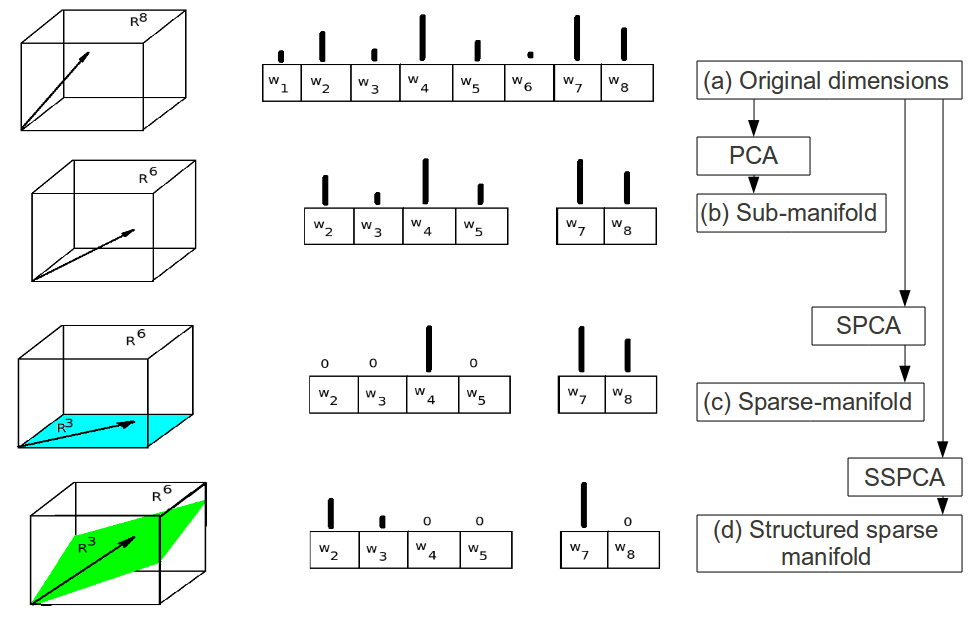
\includegraphics[width=\textwidth]{./GroupSparse/figures/sspcaConcept.png}
 \caption[Conceptual illustration of structure sparse sub-manifold dictionary]{Conceptual illustration of structure sparse sub-manifold dictionary. A feature vector $\mathbf{z} \in \mathds{R}^{8}$ is projected to a sub-manifold $\mathcal{S}_{PCA} \in \mathds{R}^{6}$ using PCA. The vector $\hat{\mathbf{z}}_{PCA}$ is not the true $\mathbf{z}$, which is embedded in some other sub-manifold of a different dimensionality than $\mathcal{S}_{PCA}$. SPCA is used to represent $\mathbf{z}$ using a $\mathds{R}^{3}$-dimensional sub-manifold in $\mathbf{R}^{6}$. While SPCA, is able to estimate the true dimensionality of $\mathbf{z}$, the sub-spaces that SPCA selects are not semantically relevant. Consequently, $\hat{\mathbf{z}}_{SPCA}$ is not the true $\mathbf{z}$. SSPCA computes $\hat{\mathbf{z}}_{SSPCA}$ by representing $\mathbf{z}$ using a semantically relevant sub-manifold $\mathcal{S}_{SSPCA}$. The subspaces that constitute $\mathcal{S}_{SSPCA}$ are sparse and semantically relevant simultaneously. This allows $\hat{\
mathbf{z}}_{SSPCA}$ to be the best estimate of the true $\mathbf{z}$.}
 \label{fig:sspcaconcept}
\end{figure}

Similar to the formulation of SPCA, $n$ feature vectors $\mathbf{z} \in \mathds{R}^{p}$ are utilized to compute the dictionary $\mathbf{D}$ of $r$ elements. The feature vectors are in matrix $\mathbf{Z} \in \mathds{R}^{p \times n}$. The empirical risk of a dictionary element $\mathbf{d} \in \mathds{R}^{p}$ for the $n$ feature vectors is $\frac{1}{n} \sum_{i=1}^{n} L(\mathbf{z}_{i}, \mathbf{d} \alpha_{i})$. Co-clustering is utilized to compute groups of subspaces $\mathcal{G}$, which was described in \cref{ch_coclustering_sec_groupingmanifolds}. The groups account for all the subspaces of the descriptor, so $\cup_{G \in \mathcal{G}} G = \{1, \ldots, p \}$. The regularization term $\Omega$ using this group structure, based on \citep{Jenatton2010}, is

\begin{equation}
\begin{array}{ll}
 \Omega(\mathbf{d}) &= \sum_{G \in \mathcal{G}} (\sum_{j \in G} (d_{j}^{G})^{2} |\mathbf{d}_{j}|^{2} )^{\frac{1}{2}} \\
                    &= \sum_{G \in \mathcal{G}} \parallel d^{G} \circ \mathbf{d} \parallel_{2}
 \end{array}
\end{equation}

where the term $(d^{G})_{G \in \mathcal{G}}$ serves as a indicator vector; a $|\mathcal{G}|$-tuple $p$-dimensional vector, such that $d_{j}^{G} > 0$ if $j \in G$ and $d_{j}^{G} = 0$ otherwise. The regularization problem is

\begin{equation}
 \min \frac{1}{2} \parallel \mathbf{Z} - \mathbf{D} \mathbf{A} \parallel^{2} + \lambda \sum_{G \in \mathcal{G}} \parallel d^{G} \circ \mathbf{d} \parallel_{2}
\end{equation}

The regularization term $\Omega(\mathbf{d}) = \sum_{G \in \mathcal{G}} \parallel d^{G} \circ \mathbf{d} \parallel_{2}$ is a mixed $\ell_{2,1}$-norm \citep{Zhao2009}. At the group level, it functions like an $\ell_{1}$-norm and consequently $\Omega(\cdot)$ induces group sparsity. In other words, each $d^{G} \circ \mathbf{d}$ is encouraged to be zero. In contrast, within the groups $G \in \mathcal{G}$, the $\ell_{2}$-norm does not encourage sparsity. Intuitively, for a certain subset of groups $\mathcal{G}' \subseteq \mathcal{G}$, the vectors $\mathbf{d}_{G}$ associated with the groups $G \in \mathcal{G}'$ will be exactly equal to zero, leading to a set of zeros which is the union of these groups $\bigcup_{G \in \mathcal{G}'} G$. The set of allowed zero patterns should be the union-closure of $\mathcal{G}$: $\mathcal{Z} = \{ \cup_{G \in \mathcal{G}'} G \mbox{ ; } \mathcal{G}' \subseteq \mathcal{G} \}$. The complementary non-zero patterns are : $\mathcal{P} = \{ \cap_{G \in \mathcal{G}'} G^{c} \mbox{ ; } \
mathcal{G}' \subseteq \mathcal{G} \}$.

\subsection[Evaluating Structured Subspace Dictionary]{Evaluating Structured Sparse Subspace Dictionary}
\label{ch_groupsparse_subsec_eval_structuremanifold}

In the experiments in this section, the datasets used are VOC-2006, VOC-2007. The image feature descriptor used is dense-SIFT. In the dense sampling, the descriptor patch size was $8 \times 8$ pixels with a step size of $4$ pixels. All the images were converted to grey scale. The implementation of SIFT in \citep{Vedaldi2008} was used. Similar to the experiments in previous chapters, the training and test set were the train and validation set provided for VOC-2006, and VOC-2007 in \citep{pascalvoc2006}, and \citep{pascalvoc2007} respectively. 

A random sample of size $100000$ feature vectors is collated from the images in the training set. It is used to compute co-clusters using information-theoretic co-clustering and sum-squared residue co-clustering. The number of groups in this experiment is $50$. The estimated groups are utilized as a priori structure for the group regularization term in SSPCA. The dictionary size is $1000$, which is in keeping with previous experiments. The sparse subspace dictionary uses the $\ell_{1}$-norm regularization while the structured sparse subspace dictionary uses the mixed $\ell_{2,1}$-norm regularization. The implementation of SPCA and SSPCA is based on \citep{Jenatton2009}. The optimization routine is run for a maximum of $1000$ iterations. The regularization parameter is $\lambda = 10^{-8}$. The stopping criterion for change in error is empirically determined to be $10^{-12}$. The optimization follows an alternative scheme between the dictionary and the coefficient matrices, optimizing each in turn while the other remains fixed. The number of iterations for each matrix is $5$. Similar to previous experiments, the SVM classifier with RBF kernel is used in this experiment. 

The graphs show the performance, in terms of mAP of classification for each category in each of the datasets. The results show that the structured sparse sub-manifold dictionary is better than the regular sparse sub-manifold dictionary for a majority, but not all, of the categories in each of the datasets.The results for VOC-2006 using ITCC is reported in \cref{fig:sspca2006i}, where the structured sparse dictionary performs better for $6$ of the $10$ categories. Results using SSRCC is reported in \cref{fig:sspca2006r}, where the structured sparse dictionary performs better for $5$ categories. Similarly, the results for VOC-2007 using ITCC is shown in \cref{fig:sspca2007i}, where structured sparse dictionary is better for $14$ of $20$ categories. In the results using SSRCC is shown in \cref{fig:sspca2007r}, the structured sparse dictionary is better for $10$ categories.  The variation in performance between categories is indicative of the inherent difference in difficulty of the categories. In addition, the number of groups of sub-spaces is the same for all categories, which contributes to the performance variation. In view of the inherent difference between categories, the number of groups should be tuned to be specific to each category.

\begin{figure}
 \centering
 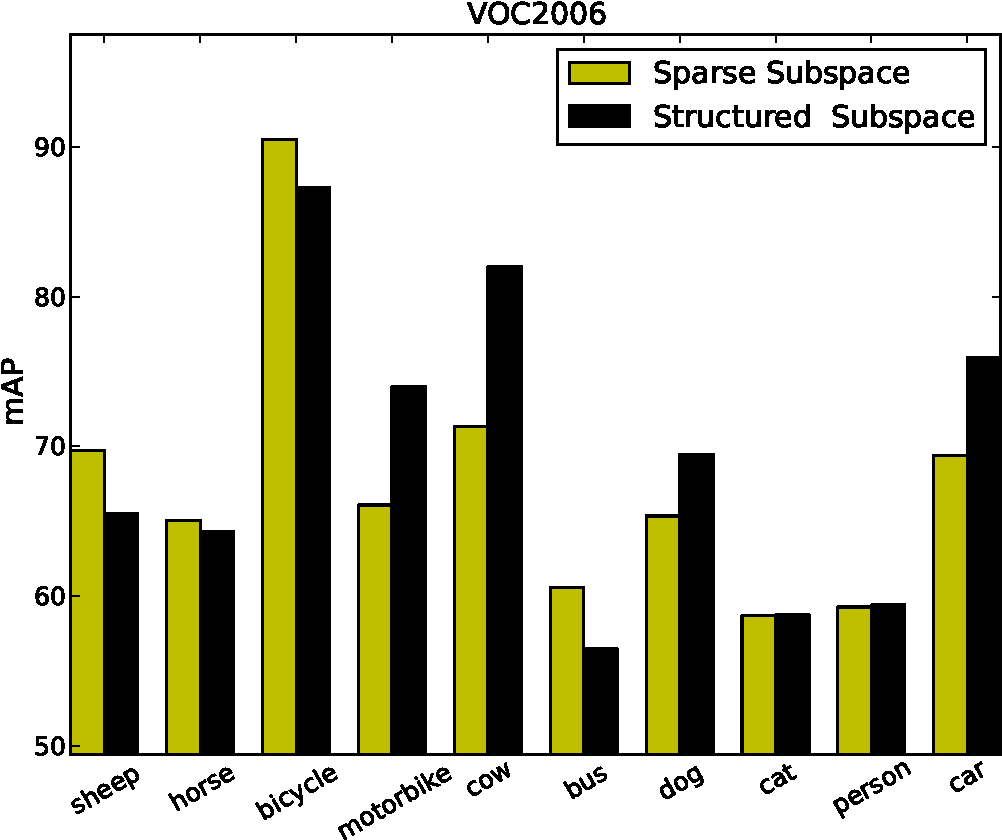
\includegraphics[width=.7\textwidth]{./GroupSparse/figures/sspca5050categoryVOC2006i-crop.pdf}
 \caption[Comparison of Sparse Subspace and ITCC Structured Sparse Subspace dictionaries using VOC-2006 dataset]{Comparative performance of Sparse Subspace and Structured Sparse Subspace dictionaries, for visual categories of VOC 2006 dataset. The graph shows the classification score measured as mAP for visual categories. The structure here is estimated using ITCC. The number of groups is $50$.}
 \label{fig:sspca2006i}
\end{figure}

\begin{figure}
 \centering
 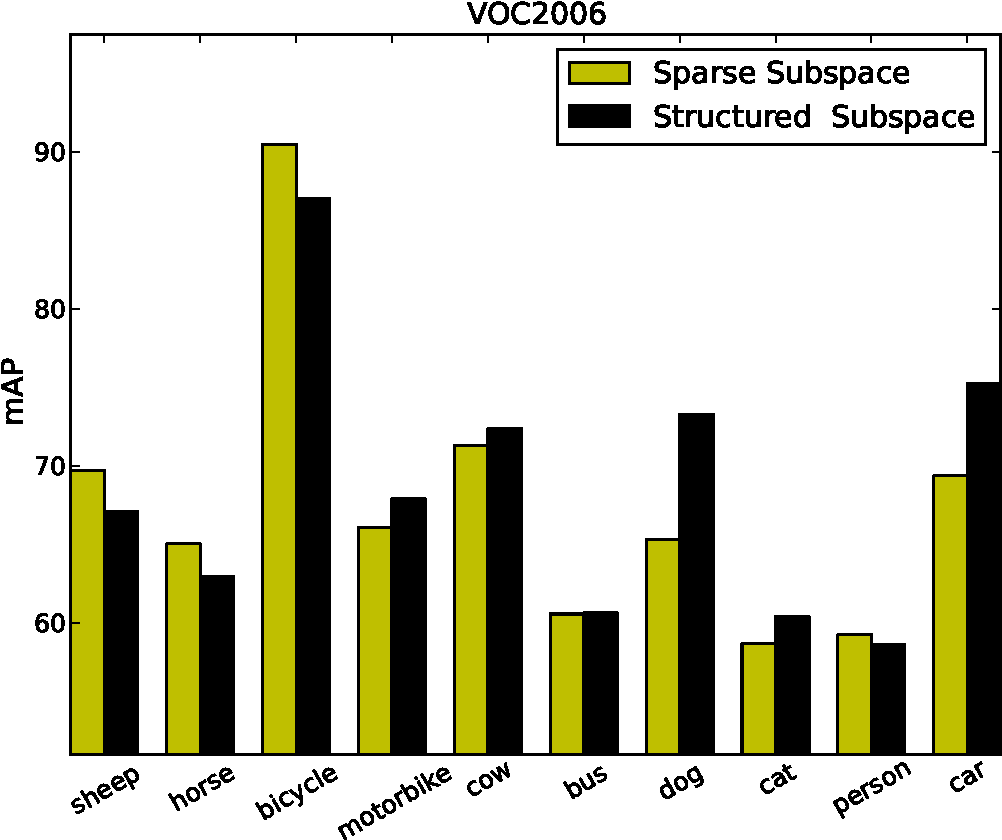
\includegraphics[width=.7\textwidth]{./GroupSparse/figures/sspca5050categoryVOC2006r-crop.pdf}
 \caption[Comparison of Sparse Subspace and SSRCC Structured Sparse dictionaries using VOC-2006 dataset]{Comparative performance of Sparse Subspace and Structured Sparse Sub-manifold dictionaries, for visual categories of VOC 2006 dataset. The graph shows the classification score measured as mAP for visual categories. The structure here is estimated using SSRCC. The number of groups is $50$.}
 \label{fig:sspca2006r}
\end{figure}

\begin{figure}
 \centering
 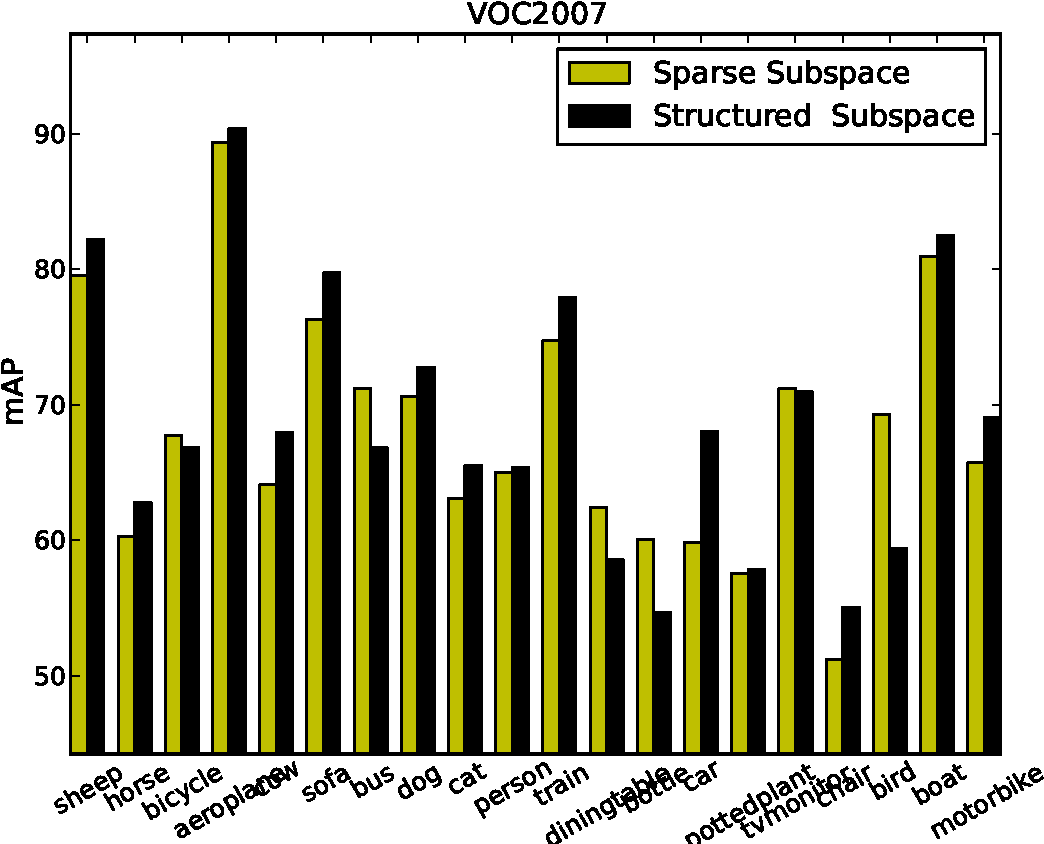
\includegraphics[width=.8\textwidth]{./GroupSparse/figures/sspca5050categoryVOC2007i-crop.pdf}
 \caption[Comparison of Sparse Subspace and ITCC Structured Sparse Subspace dictionaries using VOC-2007 dataset]{Comparative performance of Sparse Subspace and Structured Sparse Sub-manifold dictionaries, for visual categories of VOC 2007 dataset. The graph shows the classification score measured as mAP for visual categories. The structure here is estimated using ITCC. The number of groups is $50$.}
 \label{fig:sspca2007i}
\end{figure}

\begin{figure}
 \centering
 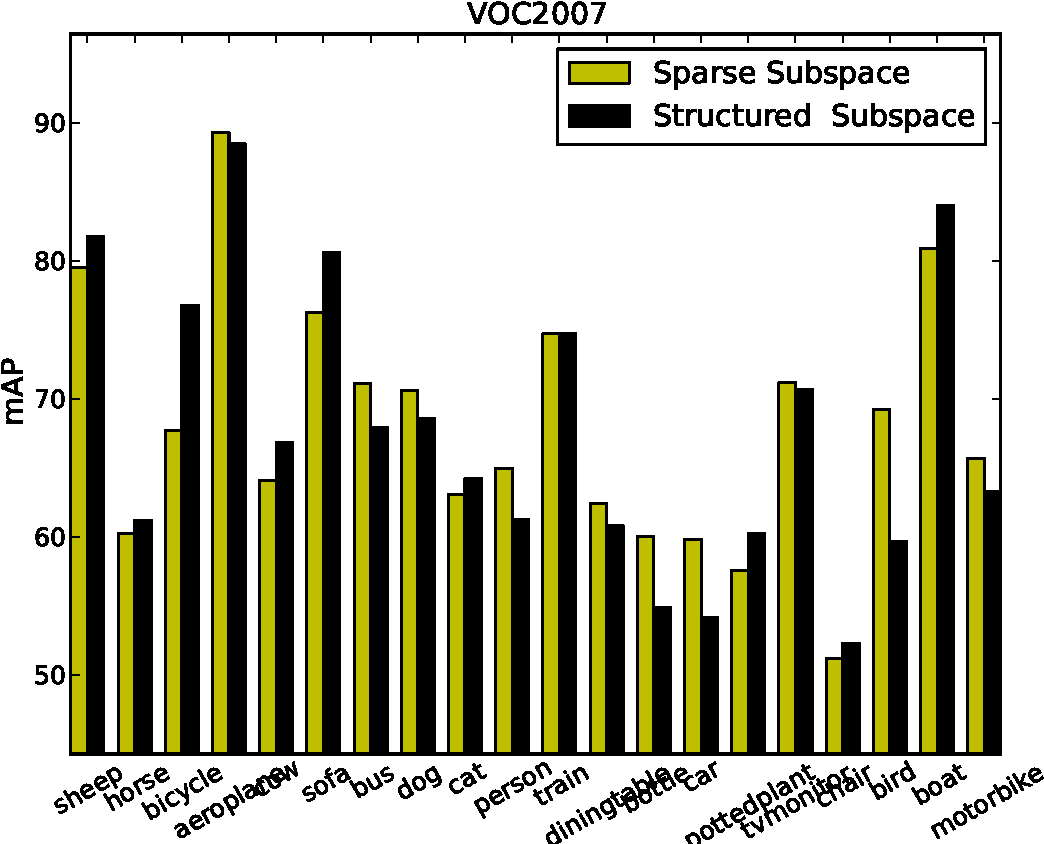
\includegraphics[width=.8\textwidth]{./GroupSparse/figures/sspca5050categoryVOC2007r-crop.pdf}
 \caption[Comparison of Sparse Subspace and SSRCC Structured Sparse Subspace dictionaries using VOC-2007 dataset]{Comparative performance of Sparse Subspace and Structured Sparse Subspace dictionaries, for visual categories of VOC 2007 dataset. The graph shows the classification score measured as mAP for visual categories. The structure here is estimated using SSRCC. The number of groups is $50$.}
 \label{fig:sspca2007r}
\end{figure}

\subsubsection{Aggregate performance across datasets}
To analyse the comparative performance of the sparse and structured sparse sub-manifold dictionaries, the aggregate classification performance across datasets is computed. The aggregate performance of each dataset is the mean of the classification score for all the categories in that dataset. This experimental setup is the same as the previous experiment. The number of groups of subspaces is $50$. The results for the VOC-2006 and VOC-2007 datasets is shown in \cref{tab:sspcaDataset}. The table shows the mean classification performance over all categories in each of VOC2006 and VOC2007 datasets. The results of structured sparse subspace dictionary using both ITCC and SSRCC is reported. The best performance for each dataset is shown in bold text. The structure sparse subspace dictionary provides a better result for both the datasets. However, for VOC2006 ITCC is comparatively better than SSRCC, whereas for VOC2007 the converse is true. The results are interesting first in that they show structure sparse 
dictionary has succeeded in incorporating semantic structure into the sub-manifolds and performed better than regular sparse subspace dictionary, and second in that the co-clustering method has a different performance for different datasets. This result emphasizes the need to use a semantic structure estimation technique that is tailored to the data distribution characteristic of a dataset. This thesis considered the K-L divergence (ITCC) and Euclidean divergence (SSRCC), but there are several popular divergences in the family of Bregman divergences that could be better alternatives. Further exploration of the family of Bregman divergences and associated co-clustering technique is left for future work.

\begin{table}[htbp]
\centering
\renewcommand{\arraystretch}{1.5}
\begin{tabular}{|l|r|c|r|}
\hline
 & \multicolumn{1}{c|}{Sparse Subspace} & \multicolumn{ 2}{c|}{Structured Sparse Subspace} \\ \hline
\multicolumn{1}{|c|}{\textit{Data Set}} & \multicolumn{1}{l|}{} & \textit{ITCC} & \multicolumn{1}{c|}{\textit{SSRCC}} \\ \hline
VOC2006 & 67.5941 & \multicolumn{1}{r|}{\textbf{70.8295}} & 68.5808 \\ \hline
VOC2007 & 67.9971 & \multicolumn{1}{r|}{68.0783} & \textbf{68.3718} \\ \hline
\end{tabular}
\caption[Aggregate classification performance of Sparse Subspace and Structured Sparse Subspace dictionaries for VOC2006 and VOC2007 datasets.]{Aggregate classification performance of Sparse Subspace and Structured Sparse Subspace dictionaries for VOC2006 and VOC2007 datasets. The table shows the mean classification performance over all categories in each of VOC2006 and VOC2007 datasets. The results of structured sparse subspace dictionary using both ITCC and SSRCC is reported. The best performance for each dataset is shown in bold text.}
\label{tab:sspcaDataset}
\end{table}


\section[Structured Sparse Encoding]{Structured Sparse Encoding}
\label{ch_groupsparse_sec_encoding}

There are two key insights that motivate the development of structured sparse encoding. The experiments in \cref{ch_coclustering_sec_structdictionary} indicated the existence of structure in the dictionary, in terms of groups of semantically related dictionary elements. The second insight is that feature vector distribution is idiomatic to a visual category. The experiments in \cref{ch_coclustering_subsubsec_evalmssdict} and \cref{ch_coclustering_subsubsec_evalstructdict} indicate that feature vectors associated with a visual category are predominantly located in a group of disjoint regions of feature space. To model such a distribution requires a parsimonious encoding scheme that can learn to represent an image using the appropriate disjoint regions only. Sparse coding methods can potentially achieve this model, provided the number of related disjoint partitions are known a priori and these appropriate partitions are selected. Sparsity is induced by use of a regularization constraint on the learnt 
coefficients. The choice of regularization scheme is important for the type of sparsity achieved, which is elaborated upon in \cref{ch_groupsparse_subsec_Lasso}. 

Notwithstanding the success of sparse regularization methods, there is an unresolved issue. Sparse models succeed in selecting the appropriate number of dictionary elements, but minimization of the loss function alone is not sufficient to guarantee selection of the appropriate subset of dictionary elements. In addition, the result of the optimization is unstable, since a small perturbation in the optimization routine could yield a different subset of dictionary elements for the representation of the same image. The reason for this issue is that these methods treat each dictionary element individually, so existing relationships and structures between these dictionary elements is disregarded. In order to reduce the instability in the selection, a potential solution is grouping dictionary elements. An appropriate grouping would consist of semantically related dictionary elements. This encourages the representation of an image using only those dictionary elements that are semantically relevant for that image. 
The method to achieve this structured selection of dictionary elements is discussed in \cref{ch_groupsparse_groupsparsecoding}, following an overview of regular sparse coding.

\subsection[Sparse Coding]{Sparse Coding}
\label{ch_groupsparse_subsec_Lasso}

Based on \citep{Aharon2006}, for training feature vectors $\mathbf{Z} \in \mathds{R}^{p \times n}$, sparse coding with the $\ell_{1}$-norm solves the problem

\begin{equation} \label{eq:l1lossfn}
 \min_{\alpha \in \mathds{R}^{p}} \parallel \mathbf{Z} - \mathbf{D} \mathbf{A} \parallel^{2} + \lambda \parallel \mathbf{A} \parallel_{1}
\end{equation}

where $\lambda$ is a regularization parameter. During dictionary learning this is a joint optimization problem with respect to dictionary $\mathbf{D}$ and the sparse coefficients $\mathbf{A} = \{\alpha^{1}, \ldots, \alpha^{r} \} \in \mathds{R}^{p \times r}$. To prevent $\mathbf{D}$ from attaining arbitrarily large values, the columns of $\mathbf{D}$ are constrained to have an $\ell_{2}$-norm less than a specified threshold - typically $\parallel \mathbf{d} \parallel_{2} \leq 1$. The canonical strategy for the joint optimization is to alternate between the two variables; keeping one fixed while minimizing the other.

The regularization problem in \cref{eq:l1lossfn} is solved to compute a dictionary matrix $\mathbf{D}$ or coefficient matrix $\mathbf{A}$. When learning a visual model, sparse coding is typically used to first compute a dictionary, where $\mathbf{Z}$ is random sample of training descriptors for the dataset \citep{Rigamonti2011, Donoho2003}. The learnt dictionary is used next to compute encoded representations of an image by computing $\mathbf{A}$, where $\mathbf{Z}$ is set of descriptors from that image \citep{Guillermo2010, Coates2011, Kreutz-Delgado2003a}. $\lambda$ is a non-negative parameter controlling the trade-off between data fitting and regularization \citep{Lee2009}. A typical convex formulation is the $\ell_{1}$-decomposition problem \citep{Donoho2003}, also known as the Lasso \citep{Tibshirani1994}:

\begin{equation}
 min_{\alpha \in \mathds{R}^{p}} \frac{1}{2} \sum_{i=1}^{n} \parallel \mathbf{z}_{i} - \mathbf{D} \alpha \parallel^{2}_{2} + \Omega(\alpha)
\end{equation}

When the value of $\lambda$ is large, $\alpha$ is known to be sparse, and only a few dictionary elements are involved. Although the use of $\ell_{1}$-norm is predominant, a natural choice would be to take the $\ell_{0}$ pseudo-norm that counts the number of non-zero coefficients in $\alpha$. Conceptually, an image should be represented by a subset of the dictionary elements. In other words, those dictionary elements that do not pertain to a visual category should not be involved in the representation of the coefficient matrix $\mathbf{A}$. However, solving the equation above in this setting is often intractable, such that one has either to look for an approximate solution using a greedy algorithm, or resort to a convex relaxation \citep{Gregor2010}.

A method closely related to Lasso was proposed by \citet{Efron2004} called Least Angle Regression Selection (LARS). Both these methods operate in two stages. The first step is to build a solution path indexed by a certain tuning parameter. In the next step the model is selected on the solution path by either cross-validation or use of some criterion. The solution paths for both Lasso and LARS are shown in \citep{Efron2004} to be piecewise linear, which renders them computationally efficient. A comparative analysis of this was provided by \citet{Rosset2007}. 

\subsection[Group Sparse Coding]{Group Sparse Coding}
\label{ch_groupsparse_groupsparsecoding}

There are a couple of issues with the Lasso and LARS methods. Although they have excellent performance and computational efficiency, they are designed for selecting individual dictionary elements. They can not be utilized for general factor selection in \cref{eq:l1lossfn}. In other words they are transparent to structure in the dictionary. So, they tend to make selections based on the strength of individual derived dictionary element rather than the strength of groups of dictionary elements (or topics), often resulting in selecting more factors than necessary. Another drawback of using the Lasso and LARS in \cref{eq:l1lossfn} is the dependency of the solution upon how the factors are orthogonalised. This is undesirable since the solution to a factor selection and estimation problem should not depend on how the factors are represented \citep{Yuan2006}. Evidently these methods require an extension that considers the dictionary elements with a pre-defined structure. The group Lasso and group LARS \citep{
Yuan2006, Bach2008} are popular choices for this extension. 

In a nutshell, the dictionary elements are assumed to be clustered in groups, and instead of summing the absolute values of each individual coefficient, the sum of Euclidean norms of the coefficients in each group is used. Intuitively, this should drive all the coefficients in one group to zero together, and thus lead to group selection \citep{Yuan2006}. In other words, the group Lasso essentially replaces groups of size one by groups of size larger than one.

Following from \cref{ch_groupsparse_subsec_Lasso} and based on \citep{Yuan2006}, the loss function for group Lasso augments \cref{eq:l1lossfn} with the additional inclusion of group information of the dictionary elements. The feature vectors $\{\mathbf{z}_{1}, \ldots, \mathbf{z}_{n}\}$ are in matrix $\mathbf{Z} \in \mathds{R}^{p \times n}$. A dictionary $\mathbf{D} \in \mathds{R}^{p \times r}$ for size $r$ has been learnt by one of the techniques discussed in \cref{ch_encoding_sec_dictionarylearning}. The elements of $\mathbf{D}$ are grouped into $k$ groups, using co-clustering as discussed in \cref{ch_coclustering_subsec_approach}. The number of elements in each group are $\{t_{1}, \ldots, t_{k} \}$, where $\sum_{i=1}^{k} t_{i} = r$. As in previous section, the coefficient matrix is $\mathbf{A} \in \mathds{R}^{r \times n}$. Consider positive definite matrices $\{K_{1}, \ldots, K_{k} \}$ corresponding to the $k$ groups in the dictionary. For feature vectors $\mathbf{Z}$, dictionary $\mathbf{D}$, and coefficients $\mathbf{A}$, group Lasso solves the regularization problem

\begin{equation} \label{eq:lossgroupLasso}
 \min \frac{1}{2} \parallel \mathbf{Z} - \sum_{j=1}^{k} \mathbf{D}_{j} \mathbf{A}_{j} \parallel_{2}^{2} + \lambda \sum_{j=1}^{k} \parallel \mathbf{A}_{j} \parallel_{K_{j}}
\end{equation}

Adopting a similar formulation to \citep{Lin2006}, $\mathbf{D}_{j}$ and $K_{j}$ are chosen respectively to be the group of dictionary elements and the reproducing kernel of the functional space induced by the $j^{th}$ group. Note that \cref{eq:lossgroupLasso} does have a degenerate expression as Lasso in \cref{eq:l1lossfn} when all the groups contain a single dictionary element, so the cardinality of each topic is one, i.e. $t_{j} = 1 \forall j \in \llbracket1 ; k \rrbracket$. The regularization constraint here lies between $\ell_{1}$, corresponding to Lasso, and $\ell_{2}$, corresponding to ridge regression. To visualize this consider \cref{fig:groupLasso}, which shows the geometric representation of the group regularization term $\Omega = \sum_{j=1}^{k} \parallel \mathbf{A}_{j} \parallel_{K_{j}}$. As an illustrative example, consider the case where there are two groups, $k = 2$. The corresponding coefficients are $\mathbf{A}_{1}$ and $\mathbf{A}_{2} = (\mathbf{A}_{11},\mathbf{A}_{12})^{T}$. In \cref{fig:groupLasso} the double pyramid shaped structure in \textit{(a)} corresponds to $\ell_{1}$-norm, so $|\mathbf{A}_{1}| + |\mathbf{A}_{21}|+ |\mathbf{A}_{22}| = 1$, which is the Lasso regression. The sphere shaped structure in \textit{(c)} corresponds to $\ell_{2}$-norm, so $\parallel (\mathbf{A}_{1}, \mathbf{A}_{2}) \parallel = 1$, which is the ridge regression. The bi-cone shaped structure in \textit{(b)} corresponds to $\ell_{2,1}$-norm, so $ |\mathbf{A}_{1}| + \parallel \mathbf{A}_{2} \parallel = 1$, which is the group Lasso. The $\ell_{1}$ considers the coefficients individually and induces sparsity in them separately. The $\ell_{2}$-norm also considers the coefficients equally, but does not encourage sparsity. In contrast to both of these norms, the essence of $\ell_{2,1}$-norm is evident in the bi-conic geometric structure. The coefficients $\mathbf{A}_{21}$ and $\mathbf{A}_{22}$ are treated equally with $\ell_{2}$-norm applied within the group. The $\ell_{1}$-norm is used between the two groups. In other words, sparsity will be induced on $\mathbf{A}_{1}$ or the pair $(\mathbf{A}_{21},\mathbf{A}_{22})$.

\begin{figure}
 \centering
 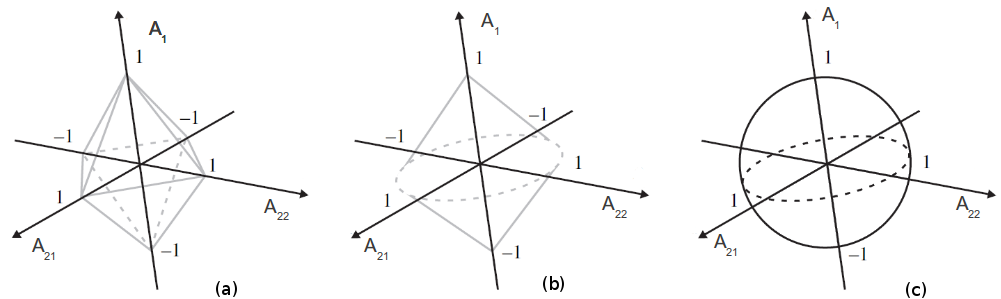
\includegraphics[width=\textwidth]{./GroupSparse/figures/grouplasso1.png}
 \caption[Pictorial representation of sparse regularization]{Pictorial representation of $\Omega = \sum_{j=1}^{k} \parallel \mathbf{A}_{j} \parallel_{K_{j}}$. In this example there are $k = 2$ groups of coefficients $\mathbf{A}_{1}$ and $\mathbf{A}_{2}$. \textit{(a)} $\ell_{1}$-norm and Lasso regression, where $|\mathbf{A}_{1}| + |\mathbf{A}_{21}|+ |\mathbf{A}_{22}| = 1$. \textit{(b)} $\ell_{2,1}$-norm and group Lasso regression, where $ |\mathbf{A}_{1}| + \parallel \mathbf{A}_{2} \parallel = 1$. \textit{(c)} $\ell_{2}$-norm and ridge regression, where $\parallel (\mathbf{A}_{1}, \mathbf{A}_{2}) \parallel = 1$.}
 \label{fig:groupLasso}
\end{figure}

\subsection[Evaluating Structured Encoding]{Evaluating Structured Sparse Encoding}
\label{ch_groupsparse_subsec_eval_structuredencoding}

\begin{figure}
 \centering
 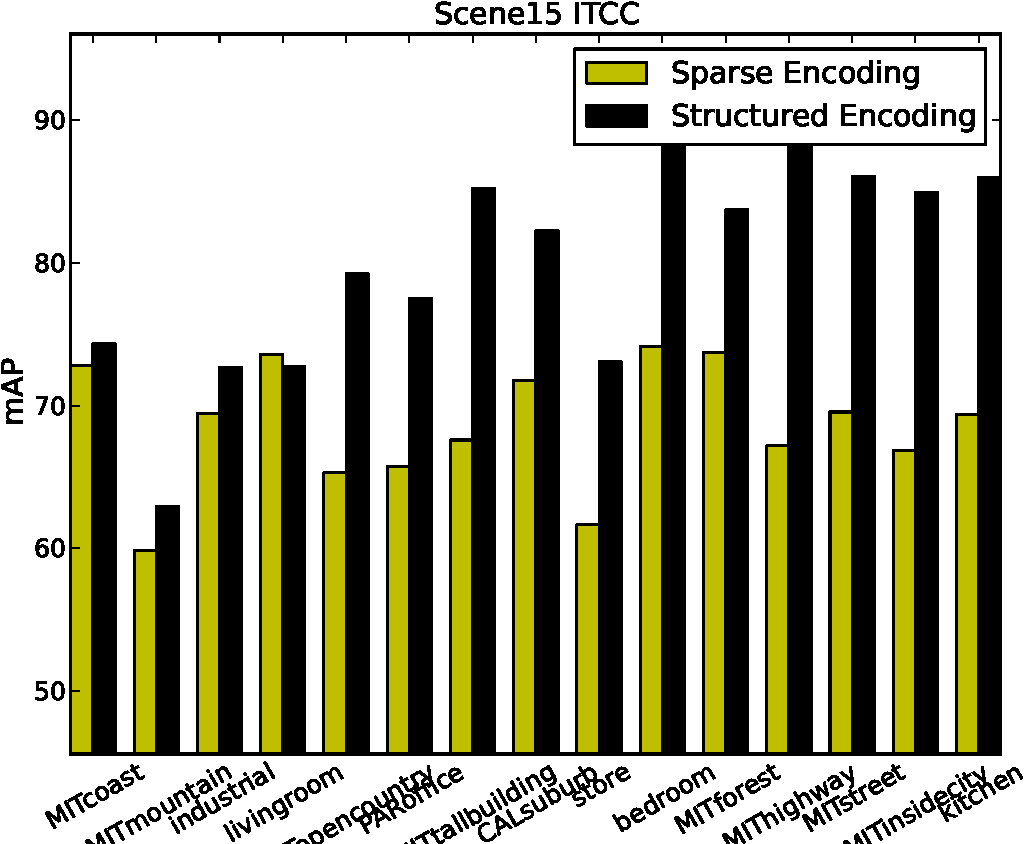
\includegraphics[width=0.7\textwidth]{./GroupSparse/figures/grouplasso1l2Scene15i-crop.pdf}
 \caption[Comparison of sparse and ITCC structured sparse coding using Scene-15 dataset]{Comparative performance of Sparse Encoding and Structured Sparse Encoding, for visual categories of Scene-15 dataset. The graph shows the classification score measured as mAP for visual categories. The structure here is estimated using information theoretic co-clustering. The number of groups is $100$ from a $1000$ element dictionary.}
 \label{fig:groupLassoScene15i}
\end{figure}

\begin{figure}
 \centering
 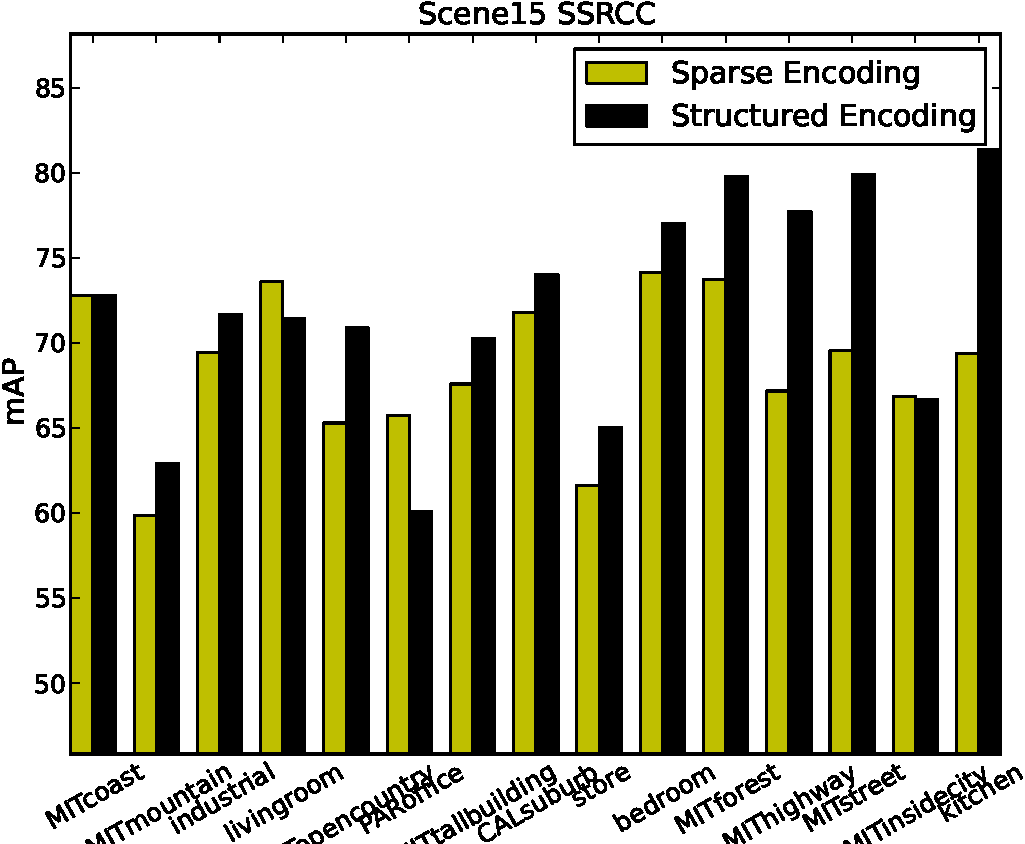
\includegraphics[width=0.7\textwidth]{./GroupSparse/figures/grouplasso1l2Scene15r-crop.pdf}
 \caption[Comparison of sparse and SSRCC structured sparse coding using Scene-15 dataset]{Comparative performance of Sparse Encoding and Structured Sparse Encoding, for visual categories of Scene-15 dataset. The graph shows the classification score measured as mAP for visual categories. The structure here is estimated using sum-squared residue co-clustering. The number of groups is $100$ from a $1000$ element dictionary.}
 \label{fig:groupLassoScene15r}
\end{figure}

In this experiment the Scene-15 dataset is used. Dense SIFT feature descriptors are generated following the procedure described in the previous experiment. A random sample of $100000$ feature vectors from all the images in the training set of every visual category for each dataset is used here. It is used to compute a dictionary of size $1000$, using k-means which is run for a maximum of $100$ iterations. In order to compare the sparse and structured sparse encoding schemes the choice of dictionary is based on the objective of not biasing the dictionary towards either of the encoding methods. The information-theoretic and sum-squared residue co-clustering methods are used to estimate topics of size $100$. The procedure for using co-clustering has been described in the experiments in \cref{ch_coclustering}. Sparse encoding uses the Lasso while the structured sparse uses the group Lasso. The choice of regularization parameter is $\lambda = 0.1$, based on preliminary analysis of an appropriate $\lambda$ for the data used in this experiment. The optimization routine is run for a maximum of $200$ iterations for encoding each image in the training and test sets. The choice of iterations here was based on the dual objective of allowing convergences a satisfactory encoded representation and curtailing the total time required to encode thousands of training and test images.  The classifier used is a SVM with RBF kernel and the performance is reported as mAP.

\begin{figure}
 \centering
 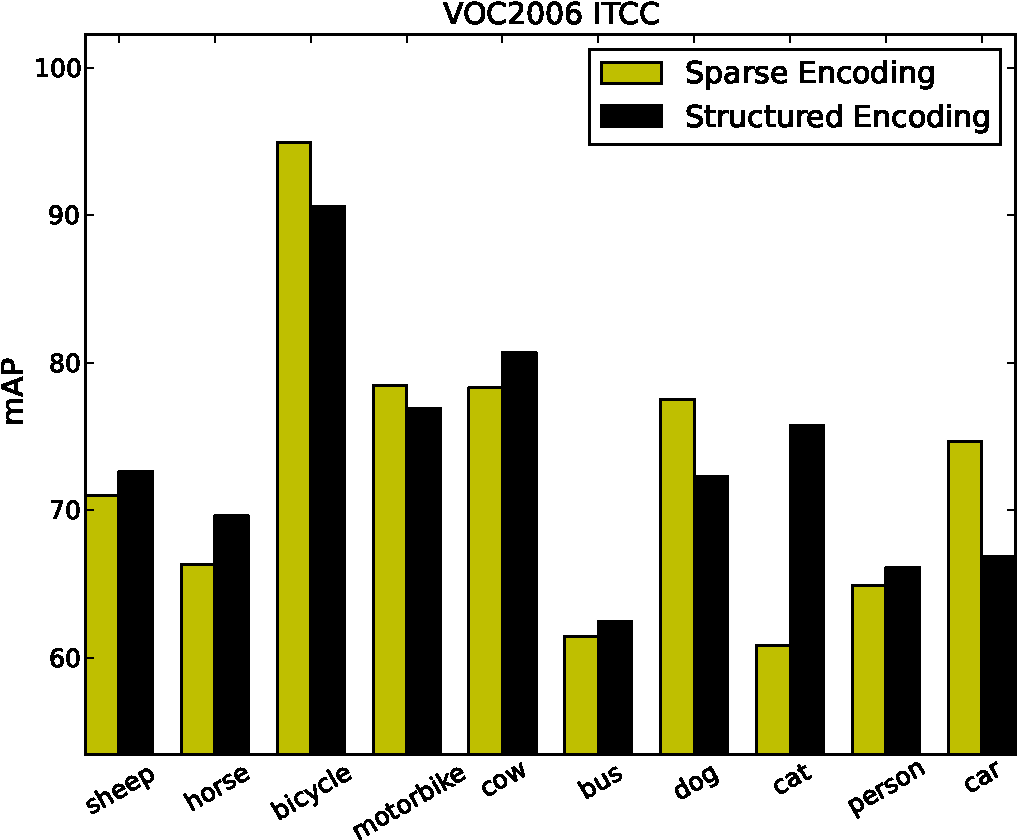
\includegraphics[width=0.7\textwidth]{./GroupSparse/figures/grouplasso1l2VOC2006i-crop.pdf}
 \caption[Comparison of sparse and ITCC structured sparse coding using VOC-2006 dataset]{Comparative performance of Sparse Encoding and Structured Sparse Encoding, for visual categories of VOC-2006 dataset. The graph shows the classification score measured as mAP for visual categories. The structure here is estimated using information theoretic co-clustering. The number of groups is $100$ from a $1000$ element dictionary.}
 \label{fig:groupLassoVOC2006i}
\end{figure}

\begin{figure}
 \centering
 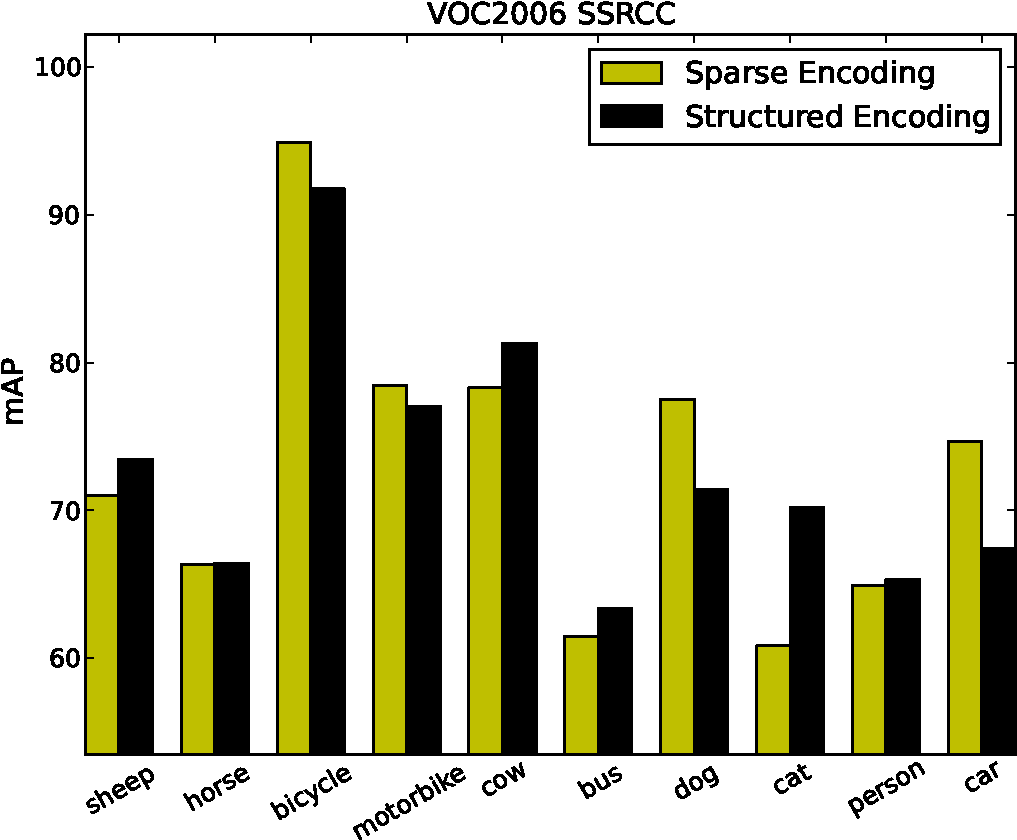
\includegraphics[width=0.7\textwidth]{./GroupSparse/figures/grouplasso1l2VOC2006r-crop.pdf}
 \caption[Comparison of sparse and SSRCC structured sparse coding using VOC-2006 dataset]{Comparative performance of Sparse Encoding and Structured Sparse Encoding, for visual categories of VOC-2006 dataset. The graph shows the classification score measured as mAP for visual categories. The structure here is estimated using sum-squared residue co-clustering. The number of groups is $100$ from a $1000$ element dictionary.}
 \label{fig:groupLassoVOC2006r}
\end{figure}

\begin{table}[htbp]
\centering
\renewcommand{\arraystretch}{1.6}
\begin{tabular}{|l|r|c|r|}
\hline
 & \multicolumn{1}{c|}{Sparse Encoding} & \multicolumn{ 2}{c|}{Structured Sparse Encoding} \\ \hline
\multicolumn{1}{|c|}{\textit{Data Set}} & \multicolumn{1}{l|}{} & \textit{ITCC} & \multicolumn{1}{c|}{\textit{SSRCC}} \\ \hline
VOC-2006 & 72.8386 & \multicolumn{1}{r|}{\textbf{73.3977}} & 72.7738 \\ \hline
Scene-15 & 68.5737 & \multicolumn{1}{r|}{\textbf{79.8794}} & 72.1155 \\ \hline
\end{tabular}
\caption[Aggregate classification performance of sparse encoding and structured sparse encoding for the VOC-2006 and Scene-15 datasets]{Aggregate classification performance of sparse encoding and structured sparse encoding for the VOC-2006 and Scene-15 datasets. The best performance for both datasets is shown in bold text. Structured sparse encoding using ITCC topic dictionary has the best comparative performance.}
\label{tab:structsparseencoding}
\end{table}

The results for Scene-15 dataset using information-theoretic co-clustering and sum-squared residue co-clustering are reported in \cref{fig:groupLassoScene15i} and \cref{fig:groupLassoScene15r} respectively. Structured sparse encoding performs better for $14$ of $15$ categories using ITCC and $11$ of $15$ categories using SSRCC. Similarly, the results for VOC-2006 dataset using ITCC and SSRCC are reported in \cref{fig:groupLassoVOC2006i} and \cref{fig:groupLassoVOC2006r} respectively, where ITCC performs better for $6$ of $10$ categories and SSRCC performs better for $6$ of $10$ categories.  With regards to the VOC-2006 dataset, structured sparse encoding has a performance comparable to regular sparse encoding. It is better for six of the ten categories in the dataset for both ITCC and SSRCC. For the Scene-15 dataset, the structured sparse encoding method has a better performance in comparison to sparse encoding for almost all of the categories. This is an encouraging result for structured learning. The aggregate performance for all categories in the dataset is reported in \cref{tab:structsparseencoding} to compare between the co-clustering methods. This is a positive result for structured sparse encoding, as the aggregate classification performance using ITCC is the best for both datasets.

These results can be interpreted as an encouraging outcome for structured learning algorithms. It should be noted that performance of structured sparse encoding depends upon several factors, including the $\ell_{1,2}$-norm regularization, the quality of the estimated groups of dictionary elements, the clustering algorithm which partitioned feature space. The $\ell_{1,2}$-norm is only one of the family of $\ell_{1,q}$-norm that could be used for enforcing group sparsity. It remains to be found if some value of $q$ other than $2$ may yield a better structured encoding. Another aspect is the dictionary size, which was kept the same across datasets. Since different datasets have different visual content, it is reasonable to expect that the appropriate dictionary size for different datasets would be different. This is one contributing factor for difference between the VOC-2006 and Scene-15 datasets. 

\section[Summary]{Summary}
\label{ch_groupsparse_sec_summary}

In this chapter, semantically related groups of basis elements estimated by co-clustering were used to augment sparsity inducing visual models with a priori semantic information.

The goal of the structured sparse subspace dictionary was to successfully incorporate the groups of subspaces estimated by the co-clustering methods to produce a dictionary that performs better than a sparse subspace dictionary without a priori structural information. The comparative performance for multiple VOC datasets in the experiments in \cref{ch_groupsparse_subsec_eval_structuremanifold} indicate that the goal has been achieved. There are some visual categories where the performance of SPCA is better. However, this result is expected in view of the significant difference between the categories in terms of inherent complexity and availability of training data to learn these complexities equally for all categories.

The aim of structured sparse encoding was to leverage the groups of dictionary elements estimated by co-clustering to encourage sparsity in the encoding of images in terms of semantically relevant topics rather than individual words. It was compared to sparse coding using $\ell_{1}$-norm, which is an excellent performing scheme. In the experiments in \cref{ch_groupsparse_subsec_eval_structuredencoding} the performance of the structured sparse encoding is marginally better than regular sparse coding when considering aggregate performance. Amongst the visual categories the comparative performance is not entirely conclusive. It should be noted that the performance of structured sparse model depends upon: the size of the dictionary and its ability to appropriately partition feature space; the presence of semantically distinct groups; and the efficacy of the co-clustering approach in estimating these groups. The presence of distinct groups is a weak hypothesis in view of the available weakly labelled data and 
relatively small training data. Therefore the results of the experiments on group structured dictionary should be considered as indicative, rather than conclusive evidence for this approach.

In the results, the performance of each category is different from other categories regardless of the method used. This suggests an inherent difference in complexity associated with each category. Of course this is not an unexpected result. One contributing factor is the tradition in the community to use the same number of training images for all categories. It is reasonable to assume that categories with a comparatively higher degree of complexity will require more training images. The number of training images has a strong bearing on the performance that can be expected from a method designed to estimate semantically relevant structure. There should be sufficient training images that span the variation in appearance in a category to allow a learning method that opportunity to learn the semantic structure. Therefore the margin of improvement of structured sparse visual model over regular sparse visual model could be attributed to lack of sufficient training data. This possibility does not itself qualify 
structured learning. Nevertheless the results of the experiments in \cref{ch_coclustering} and in \cref{ch_groupsparse} demonstrate that the methods here have succeeded in estimating semantic structure.